\appendix

\newgeometry{total={210mm,297mm},left=30mm,right=30mm,bindingoffset=5mm, top=25mm,bottom=25mm}
\begin{partwithabstract}{Appendix}
  Apendices to the document:
  \begin{enumerate}
    \item Software environment used
    \item Agreement documents for use of two datasets.
  \end{enumerate}
\end{partwithabstract}
\restoregeometry
\chapter{Medical terms}

Clarification of the medical lingo used.

\begin{SCfigure}[][htb]
  \centering
  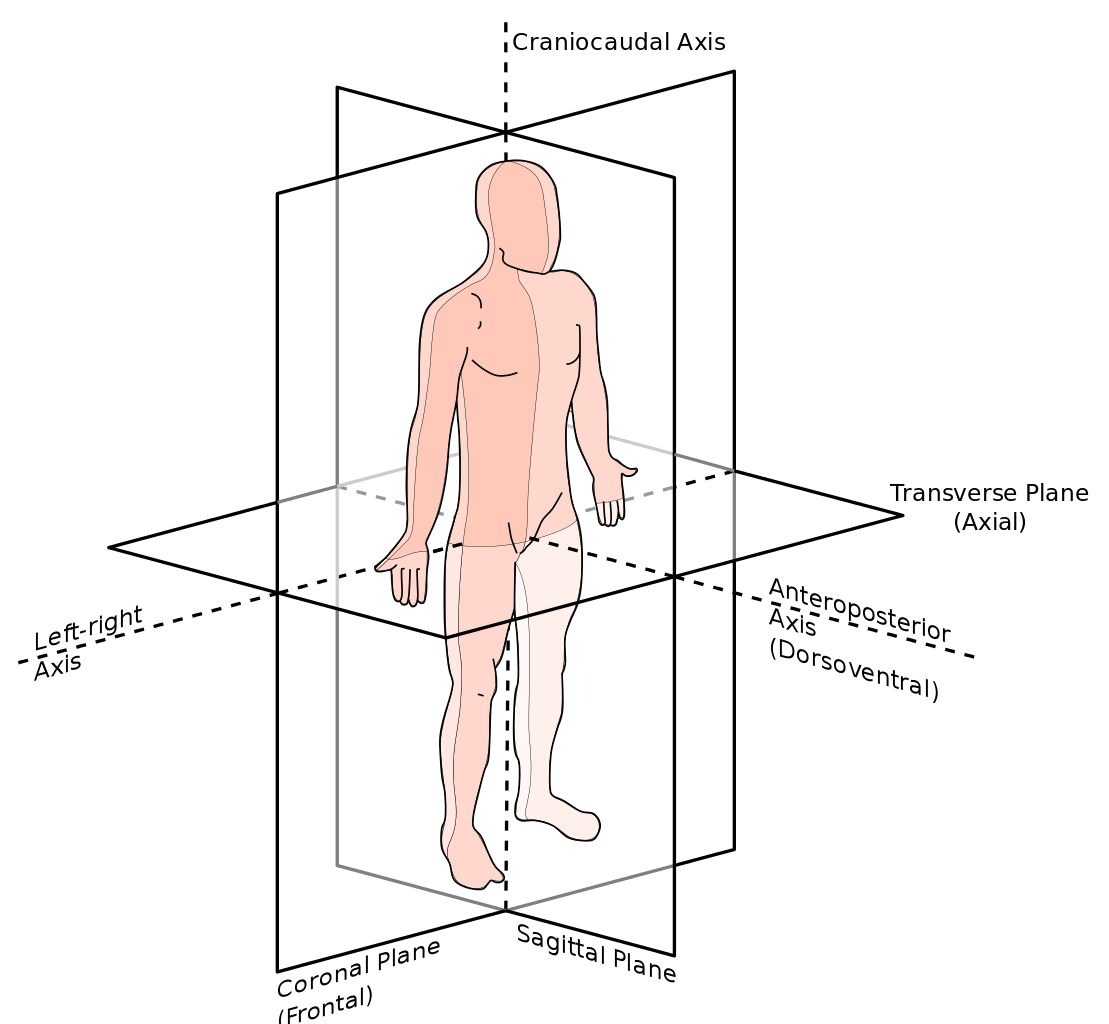
\includegraphics[width=10cm]{/home/thesis/images/Anatomical_Planes.png}
  \caption{Clarification of the terms regarding the anatomical planes
  }
\end{SCfigure}

\begin{SCfigure}[][htb]
  \centering
  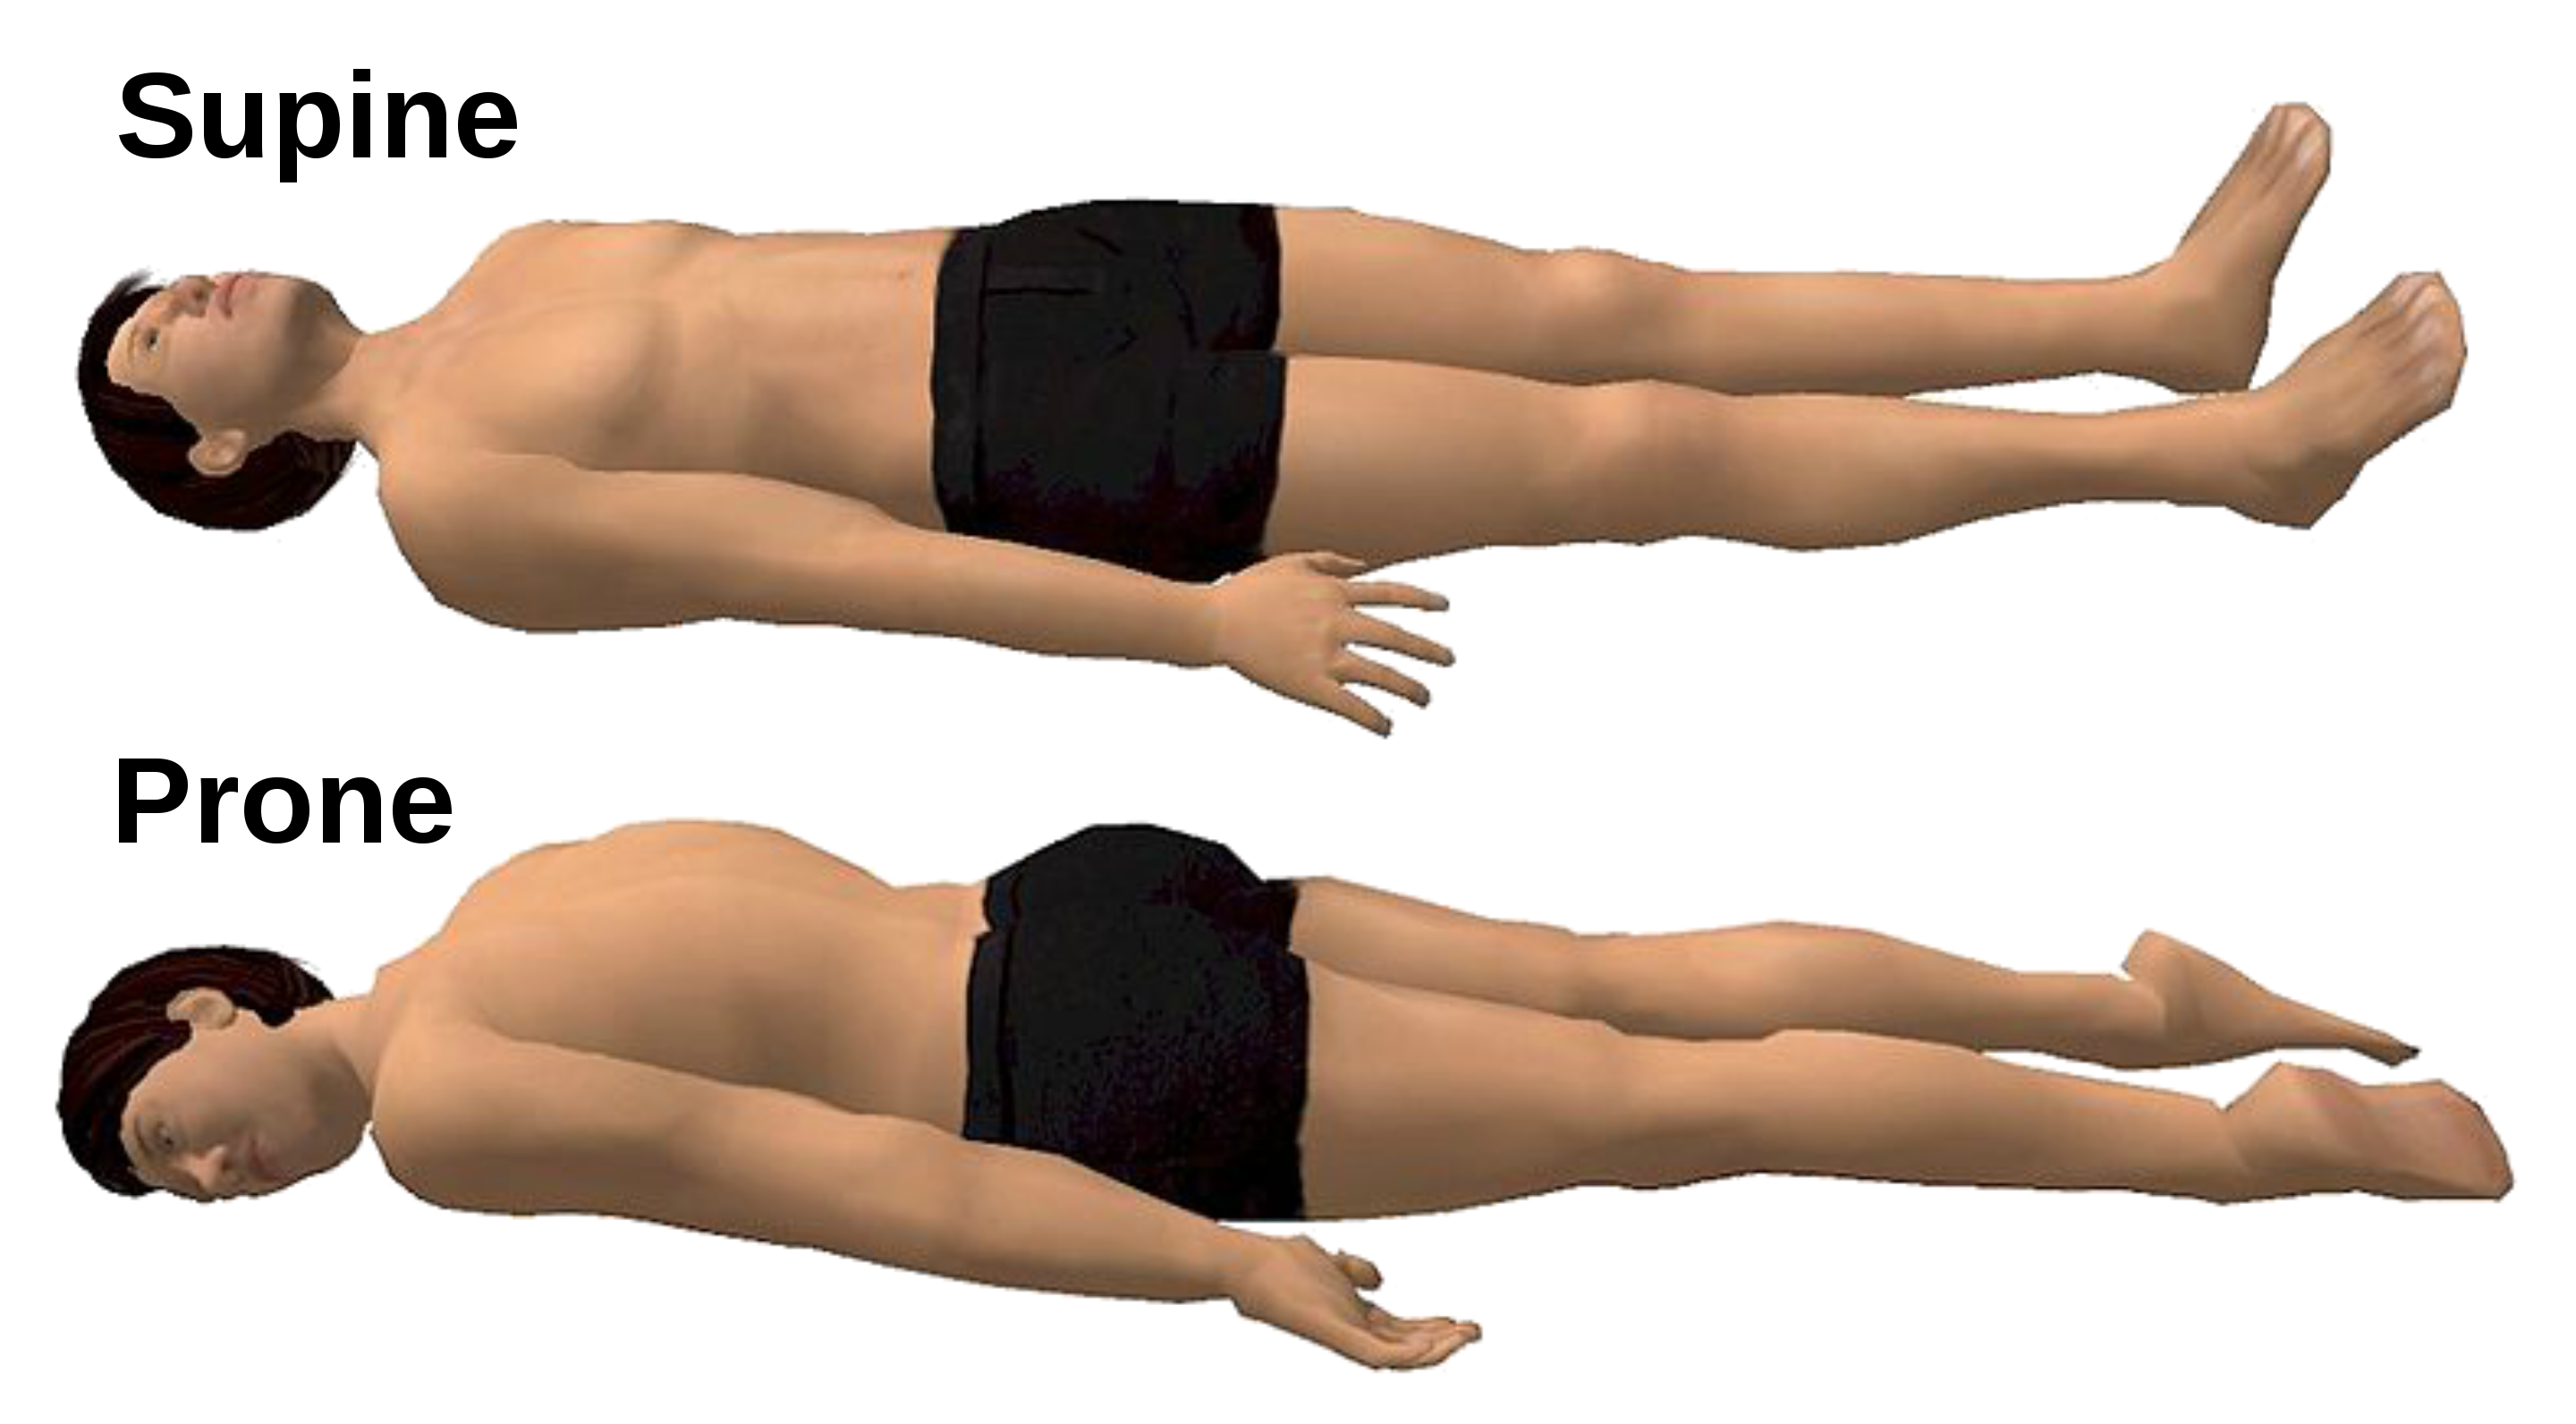
\includegraphics[width=10cm]{/home/thesis/images/prone_supine.png}
  \caption{Supine (face-up) and Prone (face-down) position of a patient.}
\end{SCfigure}

\chapter{Used software \& Reproducability of this research}

The reproducability of this work has been ensured in several ways:
\begin{description}
  \item[Data]: All datasets used in this project are publically available. For some datasets, it is required to request permission, like the author of this work has done.
  \item[Software]: This project was performed completely in python, a publically available programming language. 
  All packages used are open-source.
  To reproduce this research, no software has to be purchased. 
  \item[Code]: Both code an text of this project can be found on a public GitHub repository
  \footnote{It is possible that small adaptations of the code are required to run it on other hardware. For example, to run it using a GPU with less internal memory it could be necessary to reduce the batch size.}. 
  \item[Docker]: The specific environment to run the code mentioned above can also be found in the mentioned GitHub repository in the form a dockerfile.
  It should be noted that this dockerfile requires a GPU that supports CUDA.   
\end{description}

The above mentioned aspects should allow other researchers to reproduce the results in this document.

\todo[inline]{Software environments can be build with dockerfiles available in folder \textit{/dockerfiles/code/} of the git.}

\todo[inline]{Assure proper referencing of all libraries used}

\begin{SCtable}[\sidecaptionrelwidth][h]
 
  \begin{tabular}{ p{6cm} l l } 
   \hline
   \hline
   Library & version & reference  \\
   \hline 
   PyTorch & 1.7.1 &  \\ 
   SimpleITK &  &  \\ 
   \hline
   \hline
  \end{tabular}
  \caption{Python libraries used}

\end{SCtable}
\newgeometry{total={210mm,297mm},left=30mm,right=30mm,bindingoffset=5mm, top=25mm,bottom=25mm}
\chapter{Dataset agreements\label{seg:datasetagreement}}

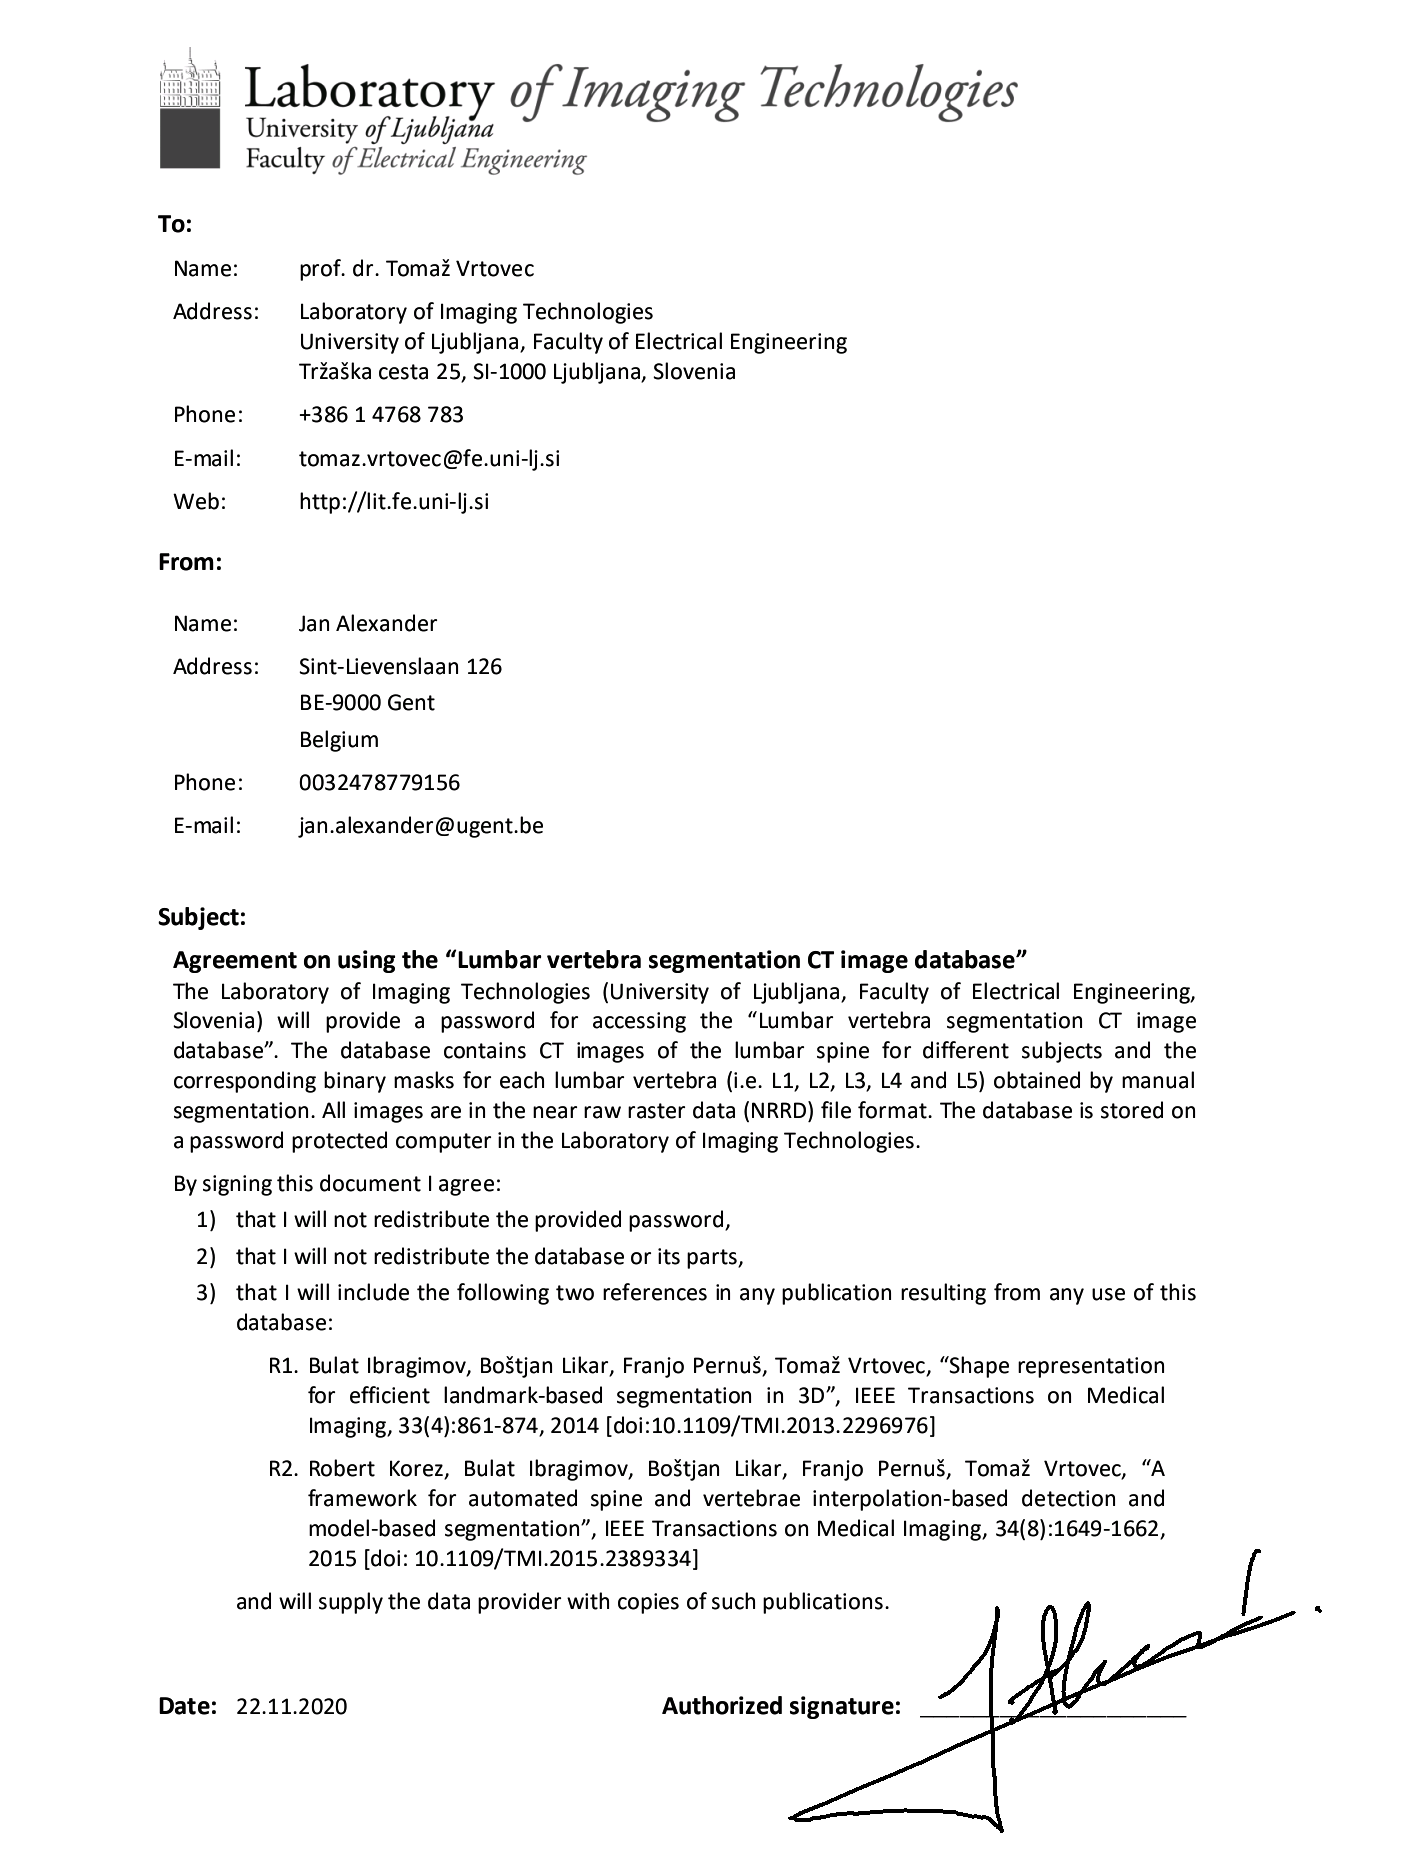
\includegraphics[width=17cm]{/home/thesis/images/AgreementxVertSeg.png}